\label{sec:comparison}

Table~\ref{tab:comparison} summarizes representative literature values for DRAM and FeRAM. 
DRAM provides high speed and very low energy/bit but requires periodic refresh due to short intrinsic retention~\cite{choi2022,kim2021_dram,iedm2023_dram}. 
FeRAM offers non-volatility with retention beyond $10^{5}$\,s and endurance reported in the $10^{12}$--$10^{13}$ range for optimized HfO$_2$ stacks, 
typically at higher write energy per bit~\cite{boscke2011,mueller2012,noheda2023,martin2020}.

\begin{table}[!t]
\centering
\caption{Representative metrics (order-of-magnitude, literature indications).}
\label{tab:comparison}
\scriptsize
\begin{tabular}{lcccc}
\toprule
Tech. & Speed (ns) & Retention (s) & Endurance & Energy/bit \\
\midrule
DRAM  & $\le 10$  & $\sim 10^{-2}$ to $10^{-1}$ & $\ge 10^{16}$ & $10$--$100$ fJ \\
FeRAM & $\le 50$  & $\ge 10^{5}$                & $10^{12}$--$10^{13}$ & $10^{2}$--$10^{3}$ fJ \\
\bottomrule
\end{tabular}
\end{table}

% ===== Figure 1: Speed (access time) vs retention =====
\begin{figure}[!t]
\centering
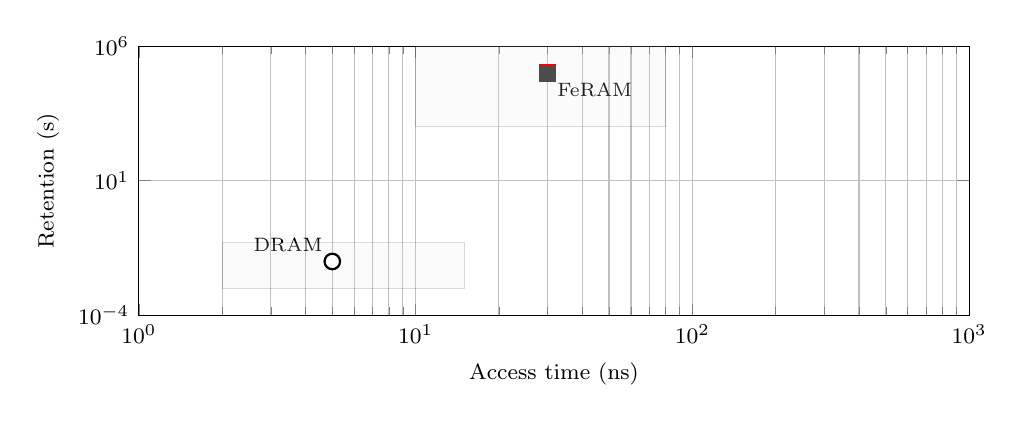
\begin{tikzpicture}
\begin{loglogaxis}[
  width=\linewidth,
  height=5.0cm,
  xlabel={Access time (ns)},
  ylabel={Retention (s)},
  xmin=1e0, xmax=1e3,
  ymin=1e-4, ymax=1e6,  % ★修正: 10^{-4}~10^{6}
  grid=both,
  label style={font=\footnotesize},
  tick label style={font=\footnotesize},
  clip=false
]

% DRAM point
\addplot+[only marks, mark=*, mark size=2.8pt,
          mark options={fill=white,draw=black,thick}]
          coordinates {(5, 1e-2)};
\node[above left, font=\scriptsize] at (axis cs:5,1e-2){DRAM};

% FeRAM point
\addplot+[only marks, mark=square*, mark size=3.0pt,
          mark options={fill=black!70}]
          coordinates {(30, 1e5)};
\node[below right, font=\scriptsize] at (axis cs:30,1e5){FeRAM};

% DRAM region
\addplot [draw=black, fill=black!10, opacity=0.15]
coordinates {(2,1e-3) (15,1e-3) (15,5e-2) (2,5e-2)} -- cycle;

% FeRAM region
\addplot [draw=black, fill=black!10, opacity=0.15]
coordinates {(10,1e3) (80,1e3) (80,1e6) (10,1e6)} -- cycle;

\end{loglogaxis}
\end{tikzpicture}
\caption{Speed vs.\ retention trade-off. DRAM is faster but requires refresh, whereas FeRAM provides long retention at modest access times.}
\label{fig:speed_retention}
\end{figure}

% ===== Figure 2: Write energy vs write time =====
\begin{figure}[!t]
\centering
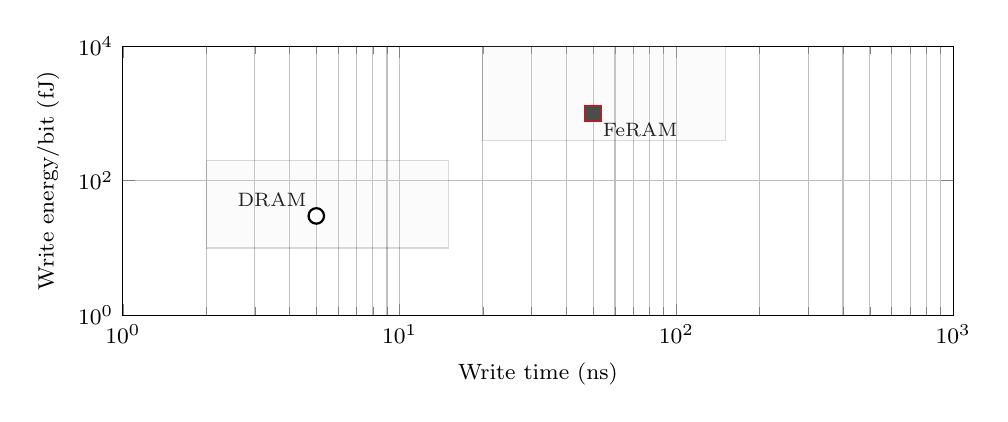
\begin{tikzpicture}
\begin{loglogaxis}[
  width=\linewidth,
  height=5.0cm,
  xlabel={Write time (ns)},
  ylabel={Write energy/bit (fJ)},
  xmin=1e0, xmax=1e3,
  ymin=1e0, ymax=1e4,  % ★修正: 10^{0}~10^{4}
  grid=both,
  label style={font=\footnotesize},
  tick label style={font=\footnotesize},
  clip=false
]

% DRAM point
\addplot+[only marks, mark=*, mark size=2.8pt,
          mark options={fill=white,draw=black,thick}]
          coordinates {(5, 30)};
\node[above left, font=\scriptsize] at (axis cs:5,30){DRAM};

% FeRAM point
\addplot+[only marks, mark=square*, mark size=3.0pt,
          mark options={fill=black!70}]
          coordinates {(50, 1000)};
\node[below right, font=\scriptsize] at (axis cs:50,1000){FeRAM};

% DRAM region
\addplot [draw=black, fill=black!10, opacity=0.15]
coordinates {(2,10) (15,10) (15,200) (2,200)} -- cycle;

% FeRAM region
\addplot [draw=black, fill=black!10, opacity=0.15]
coordinates {(20,400) (150,400) (150,1e4) (20,1e4)} -- cycle;

\end{loglogaxis}
\end{tikzpicture}
\caption{Conceptual write energy versus write time. DRAM typically achieves lower energy at short write times; FeRAM writes cost more energy but persist without refresh.}
\label{fig:energy_speed}
\end{figure}
